%% abtex2-modelo-trabalho-academico.tex, v-1.9.7 laurocesar
%% Adaptado para Atividade de Legislação - UFPA

\documentclass[
	12pt,				% tamanho da fonte
	openright,			% capítulos começam em pág ímpar
	oneside,			% impressão apenas frente
	a4paper,			% tamanho do papel
	english,			% idioma adicional para hifenização
	brazil				% o último idioma é o principal do documento
	]{abntex2}

% ---
% Pacotes básicos 
% ---
\usepackage{lmodern}			% Usa a fonte Latin Modern
\usepackage[T1]{fontenc}		% Selecao de codigos de fonte.
\usepackage[utf8]{inputenc}		% Codificacao do documento
\usepackage{indentfirst}		% Indenta o primeiro parágrafo
\usepackage{color}				% Controle das cores
\usepackage{graphicx}			% Inclusão de gráficos
\usepackage{microtype} 			% para melhorias de justificação
\usepackage{listings}			% Inclusão de código
\usepackage{xcolor}				% Cores para código
\usepackage{float}              % Posicionamento de floats
\usepackage{amsmath}            % Matemática avançada

% Configuração para listings (código)
\definecolor{codegreen}{rgb}{0,0.6,0}
\definecolor{codegray}{rgb}{0.5,0.5,0.5}
\definecolor{codepurple}{rgb}{0.58,0,0.82}
\definecolor{backcolour}{rgb}{0.95,0.95,0.92}

\lstset{
    backgroundcolor=\color{backcolour},
    commentstyle=\color{codegreen},
    keywordstyle=\color{magenta},
    numberstyle=\tiny\color{codegray},
    stringstyle=\color{codepurple},
    basicstyle=\ttfamily\footnotesize,
    breakatwhitespace=false,
    breaklines=true,
    captionpos=b,
    keepspaces=true,
    numbers=left,
    numbersep=5pt,
    showspaces=false,
    showstringspaces=false,
    showtabs=false,
    tabsize=2,
    language=Python
}

% ---
% Pacotes de citações
% ---
\usepackage[brazilian,hyperpageref]{backref}	 
\usepackage[alf]{abntex2cite}	

% --- 
% CONFIGURAÇÕES DE PACOTES
% --- 

% Configurações do pacote backref
\renewcommand{\backrefpagesname}{Citado na(s) página(s):~}
\renewcommand{\backref}{}
\renewcommand*{\backrefalt}[4]{
	\ifcase #1 %
		Nenhuma citação no texto.%
	\or
		Citado na página #2.%
	\else
		Citado #1 vezes nas páginas #2.%
	\fi}%

% ---
% Informações de dados para CAPA e FOLHA DE ROSTO
% ---
\titulo{Trabalho 1: Raízes de Equações}
\autor{Amanda Gabrielly Ribeiro da Conceição - 202363640015 \\ Breno de Medeiros Paulo - 202206840034 \\ João Victor Santos Brito Ferreira - 202207040028 \\ Livia Stefane Hipolito Pires - 202206840043 \\ Nicolas Ranniery da Silva Sousa - 202206840051}
\local{Belém}
\data{2026}
\orientador{ Prof. Dr. Jeferson Danilo Lima Silva}
\instituicao{Universidade Federal do Pará}
\instituicaounidade{Instituto de Tecnologia (ITEC)}
\instituicaosubunidade{Faculdade de Engenharia da Computação e Telecomunicações}

\tipotrabalho{Trabalho Acadêmico}

\preambulo{Relatório de Métodos Numéricos apresentado à Universidade Federal do Pará referente aos problemas de Raízes de Equações.}
% ---

% ---
% Configurações de aparência do PDF final
% ---
\definecolor{blue}{RGB}{41,5,195}
\makeatletter
\hypersetup{
		pdftitle={\@title}, 
		pdfauthor={\@author},
    	pdfsubject={\imprimirpreambulo},
	    pdfcreator={LaTeX with abnTeX2},
		colorlinks=true,       		
    	linkcolor=black,          	
    	citecolor=black,        		
    	filecolor=black,      		
		urlcolor=black,
		bookmarksdepth=4
}
\makeatother

% --- 
% Espaçamentos entre linhas e parágrafos 
% --- 
\setlength{\parindent}{1.3cm}
\setlength{\parskip}{0.2cm}  

% ---
% compila o indice
% ---
\makeindex

% ----
% Início do documento
% ----
\begin{document}

% Seleciona o idioma do documento
\selectlanguage{brazil}
\frenchspacing 

% ----------------------------------------------------------
% ELEMENTOS PRÉ-TEXTUAIS
% ----------------------------------------------------------

\imprimircapa
\imprimirfolhaderosto*

% ---
% Resumo
% ---
\setlength{\absparsep}{18pt} 
\begin{resumo}
Este trabalho apresenta o desenvolvimento, implementação e análise de algoritmos voltados à determinação de raízes de funções contínuas, incluindo métodos intervalares (Busca Incremental, Bisseção, Falsa Posição e Falsa Posição Modificada), métodos abertos (Ponto Fixo Simples, Newton-Raphson e Secante) e métodos aplicados a polinômios (Müller e Bairstow). Os algoritmos foram desenvolvidos na linguagem Python, fazendo uso intensivo das bibliotecas SymPy, NumPy e Pandas para processamento simbólico e organização de dados iterativos de convergência. Os resultados demonstram o fiel cumprimento das especificações de parada (tolerância e limite de iterações), evidenciando a comparação do perfil de convergência e robustez frente a diferentes funções-teste.

 \textbf{Palavras-chave}: Métodos Numéricos, Raízes de Equações, Bisseção, Newton-Raphson, Python.
\end{resumo}

% ---
% inserir o sumario
% ---
\pdfbookmark[0]{\contentsname}{toc}
\tableofcontents*
\cleardoublepage

% ----------------------------------------------------------
% ELEMENTOS TEXTUAIS
% ----------------------------------------------------------
\textual

% ----------------------------------------------------------
% ----------------------------------------------------------
\chapter{Introdução}
% ----------------------------------------------------------

A determinação de raízes de funções é uma tarefa fundamental em análise numérica e engenharia \cite{chapra2016,burden2015}. Muitos problemas práticos, especialmente em engenharia de telecomunicações, processamento de sinais digitais e modelagem de sistemas físicos, recaem na necessidade de resolver equações do tipo $f(x) = 0$. 

Enquanto métodos analíticos funcionam para casos simples, a maioria dos problemas reais envolve funções transcendentais ou polinômios de alta ordem que não permitem solução algébrica explícita \cite{quarteroni2007}. Portanto, métodos numéricos são essenciais para encontrar aproximações confiáveis dessas raízes dentro de uma precisão especificada.

Este trabalho apresenta uma implementação integrada de diversos métodos numéricos para determinação de raízes, organizados em três grupos principais:

\begin{enumerate}
    \item \textbf{Métodos Intervalares}: Bisseção, Falsa Posição e sua variante Modificada
    \item \textbf{Métodos Abertos}: Ponto Fixo Simples, Newton-Raphson e Secante
    \item \textbf{Métodos Polinomiais}: Müller e Bairstow
\end{enumerate}

Os algoritmos foram implementados em Python 3, utilizando bibliotecas especializadas (NumPy, SymPy, Pandas e Matplotlib) para processamento numérico, manipulação simbólica de derivadas, organização de dados iterativos e visualização gráfica interativa.

% ----------------------------------------------------------
\chapter{Metodologia}
% ----------------------------------------------------------

\section{Estrutura Geral de Implementação}

Os métodos foram desenvolvidos dentro de um \textit{Jupyter Notebook} interativo, permitindo validação contínua e visualização dos resultados. Cada método segue uma estrutura padrão:

\begin{enumerate}
    \item Entrada e validação de dados do usuário
    \item Iteração numerando com monitoramento de convergência
    \item Construção de tabelas e gráficos de saída
    \item Alertas e verificações de segurança
\end{enumerate}

A seleção de bibliotecas justifica-se como segue:

\begin{itemize}
    \item \textbf{SymPy}: Manipulação simbólica para cálculo automático de derivadas (obrigação em Newton-Raphson) \cite{sympy2024}
    \item \textbf{NumPy}: Vetorização e operações eficientes em arrays numéricos \cite{numpy2024}
    \item \textbf{Pandas}: Organização de resultados iterativos em DataFrames estruturados \cite{pandas2024}
    \item \textbf{Matplotlib}: Visualização gráfica clara e interativa \cite{matplotlib2024}
    \item \textbf{ipywidgets}: Controles interativos (sliders, botões) para exploração visual \cite{ipywidgets2024}
\end{itemize}

\section{Métodos Intervalares}

Os métodos intervalares baseiam-se na estratégia de confinamento de raízes dentro de intervalos successivamente menores \cite{ruggiero2004}. Todos requerem que a função seja contínua e mude de sinal no intervalo inicial.

\subsection{Busca Incremental de Raízes}

Implementa uma varredura do intervalo fornecido pelo usuário em $N$ subdivisões, detectando automaticamente subintervalos onde ocorrem mudanças de sinal (indicando raízes).

\textbf{Fundamento Teórico:}
O método baseia-se no Teorema do Valor Intermediário \cite{burden2015}: se $f$ é contínua em $[a,b]$ e $f(a) \cdot f(b) < 0$, então existe pelo menos uma raiz em $(a,b)$. A varredura particiona o intervalo original em $N$ subintervalos e verifica o sinal em cada ponto.

\vspace{0.3cm}

\textbf{Implementação:}

O código de entrada (Requisito 1.1) implementa:

\begin{lstlisting}[language=Python, caption={Requisito 1.1 - Entrada de Dados}]
expr_str = input("Insira a expressão da função f(x): ").strip()
intervalo_1 = float(input("Insira a primeira extremidade do intervalo: "))
intervalo_2 = float(input("Insira a segunda extremidade do intervalo: "))
N = int(input("Insira o número N de subdivisões: "))

# Validação
if intervalo_1 > intervalo_2:
    intervalo_1, intervalo_2 = intervalo_2, intervalo_1
\end{lstlisting}

\vspace{0.3cm}

O cálculo de subdivisões (Requisito 1.2) utiliza:

\begin{lstlisting}[language=Python, caption={Requisito 1.2 - Cálculo de Subdivisões}]
x = symbols('x')
expr = sympify(expr_str)
f = lambdify(x, expr, 'numpy')

pontos = np.linspace(intervalo_1, intervalo_2, N + 1)
valores_funcao = f(pontos)

dados_subdivisoes = pd.DataFrame({
    'Ponto': pontos,
    'f(x)': valores_funcao,
    'Sinal': ['Positivo' if v > 0 else 'Negativo' 
              if v < 0 else 'Zero' for v in valores_funcao]
})
\end{lstlisting}

A detecção de raízes (Requisito 1.3) ocorre através de:

\begin{lstlisting}[language=Python, caption={Requisito 1.3 - Detecção de Mudanças de Sinal}]
subintervalos_raizes = []

for i in range(len(pontos) - 1):
    if valores_funcao[i] * valores_funcao[i+1] < 0:
        # Mudança de sinal encontrada
        subintervalos_raizes.append({
            'Inicio': pontos[i],
            'Fim': pontos[i+1],
            'f(inicio)': valores_funcao[i],
            'f(fim)': valores_funcao[i+1]
        })
    elif valores_funcao[i] == 0:
        # Raiz exata detectada
        subintervalos_raizes.append({
            'Inicio': pontos[i],
            'Fim': pontos[i],
            'Tipo': 'Zero Encontrado'
        })
\end{lstlisting}

A visualização gráfica (Requisito 1.4) inclui:

\begin{lstlisting}[language=Python, caption={Requisito 1.4 - Plotagem com Destaque}]
fig, ax = plt.subplots(figsize=(12, 6))
ax.plot(x_plot, y_plot, 'b-', linewidth=2, label='f(x)')
ax.scatter(pontos, valores_funcao, color='gray', s=50, alpha=0.6)

for raiz in subintervalos_raizes:
    ax.axvspan(raiz['Inicio'], raiz['Fim'], 
               alpha=0.3, color='green')  # Destaque
    ax.scatter([raiz['Inicio'], raiz['Fim']], 
               [raiz['f(inicio)'], raiz['f(fim)']], 
               color='green', s=100, marker='o')

ax.axhline(y=0, color='black', linestyle='--', linewidth=0.8)
ax.set_title(f'Varredura de Raízes: f(x) = {expr_str}')
plt.show()
\end{lstlisting}

O refinamento iterativo (Requisito 1.5) é oferecido através de:

\begin{lstlisting}[language=Python, caption={Requisito 1.5 - Refinamento Iterativo}]
print("\nOpções:")
print("1. Refinar a busca com um novo valor de N")
print("2. Prosseguir para o cálculo de raízes")
opcao = input("\nEscolha uma opção (1 ou 2): ").strip()

if opcao == '1':
    return busca_incremental_raizes()  # Recursão
else:
    return subintervalos_raizes, expr_str
\end{lstlisting}

\vspace{0.3cm}

\textbf{Requisitos cumpridos:}
\begin{itemize}
    \item[✓] 1.1: Entrada implementada com validação de intervalo
    \item[✓] 1.2: Cálculo com $N+1$ pontos e armazenamento em DataFrame
    \item[✓] 1.3: Detecção via produto de sinais: $f(x_i) \cdot f(x_{i+1}) < 0$
    \item[✓] 1.4: Plotagem com \textit{axvspan} para destaque e cores diferenciadas
    \item[✓] 1.5: Loop recursivo permitindo ajuste de $N$ sem reiniciar
\end{itemize}

\begin{figure}[H]
    \centering
    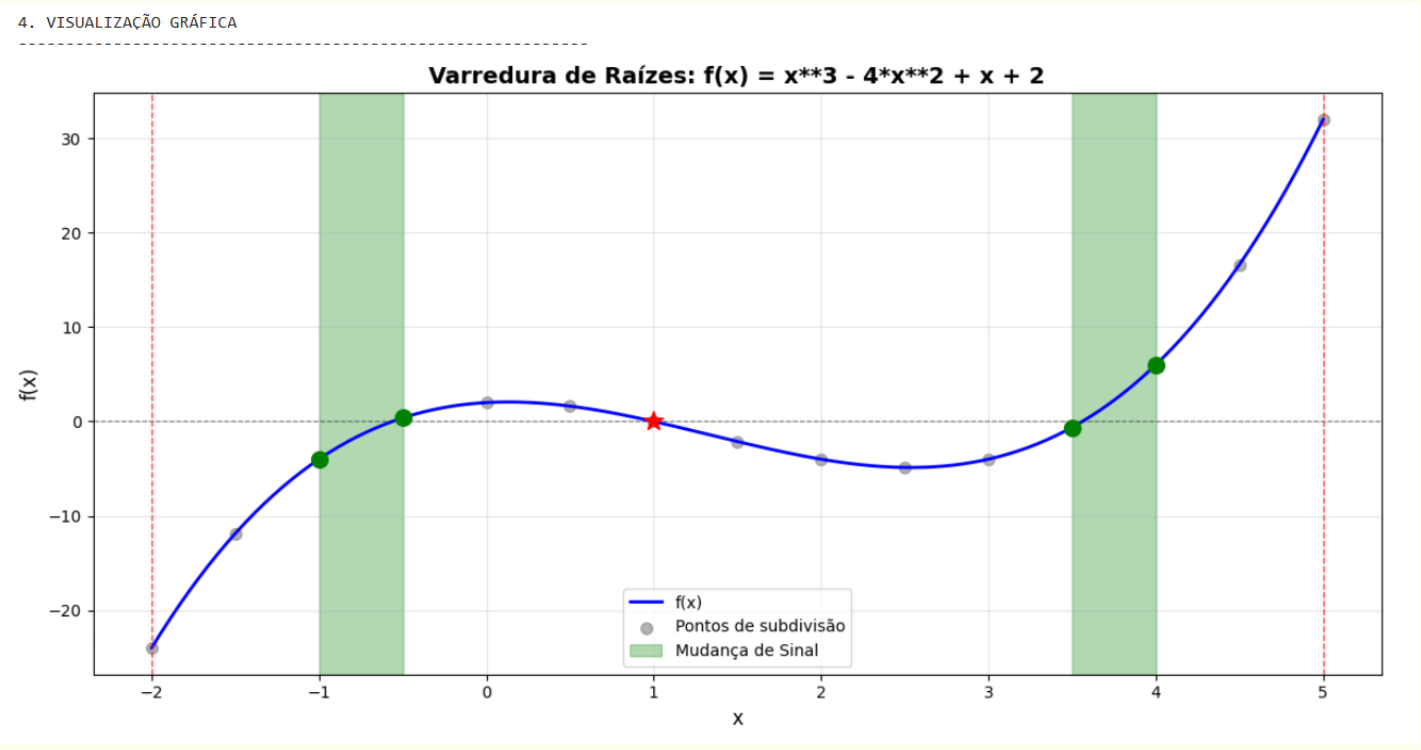
\includegraphics[width=0.8\textwidth]{assets/varredura_grafico.png}
    \caption{Visualização gráfica da varredura de raízes. Em verde são destacados os intervalos onde ocorrem mudanças de sinal, indicando a presença de raízes. Os pontos de subdivisão são marcados como referência.}
    \label{fig:varredura_grafico}
\end{figure}

\vspace{0.3cm}

\begin{figure}[H]
    \centering
    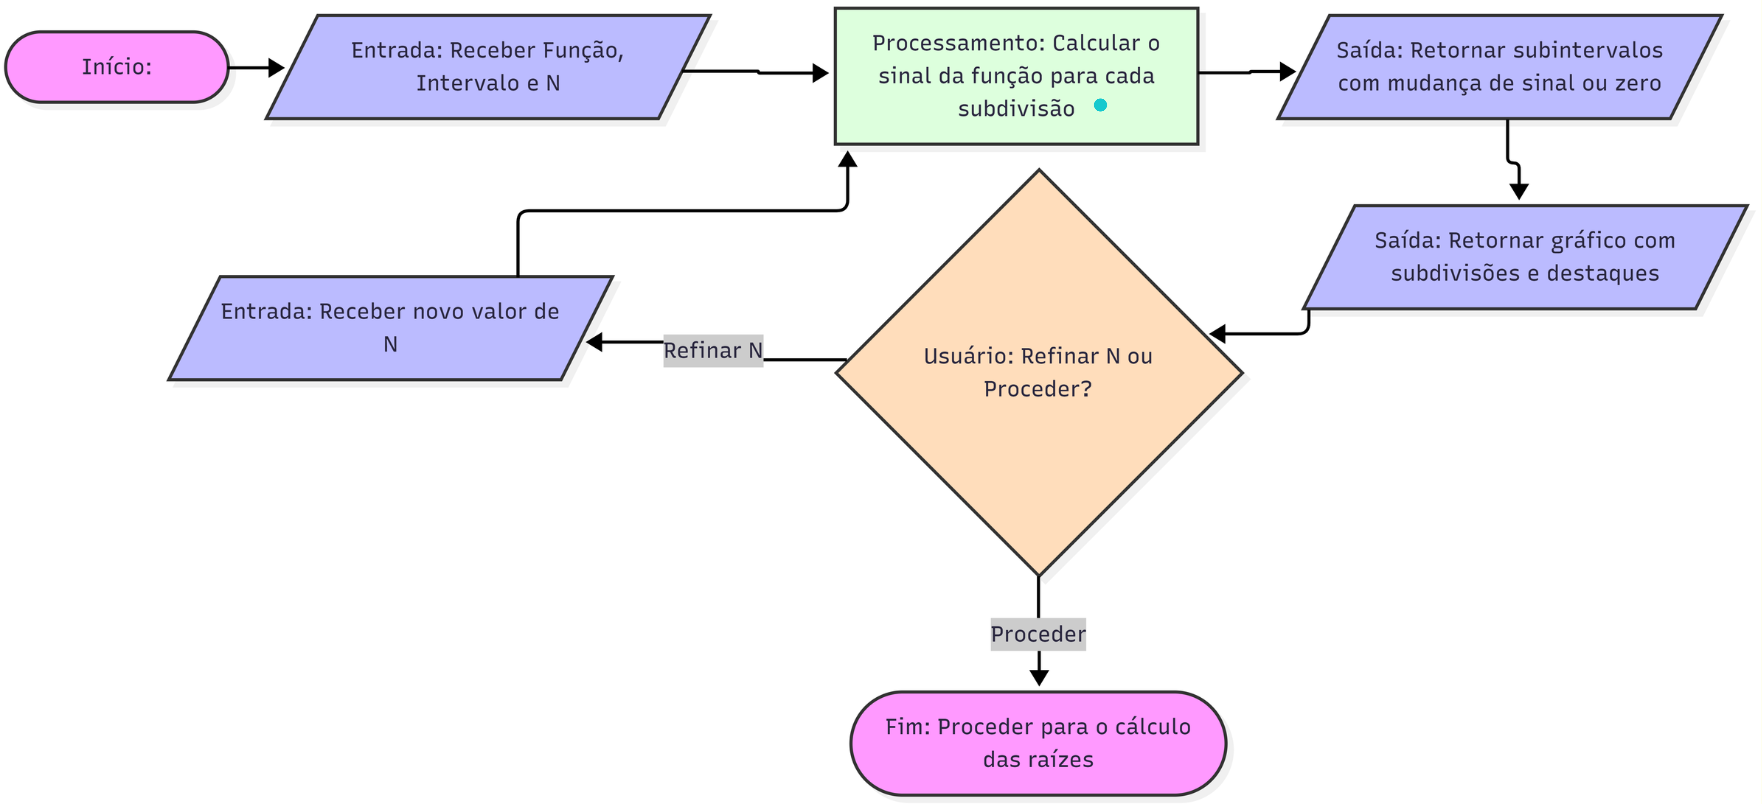
\includegraphics[width=0.8\textwidth]{assets/varredura_possiveis.png}
    \caption{Fluxograma do método}
    \label{fig:varredura_possiveis}
\end{figure}

\subsection{Método da Bisseção}

Subdivide recursivamente o intervalo $[a,b]$ no ponto médio $c$, mantendo o subintervalo contendo a raiz baseado no sinal da função \cite{burden2015,ruggiero2004}.

\textbf{Fundamento Teórico:}
Convergência garantida com taxa linear: $e_n = \frac{b_0 - a_0}{2^n}$. O número de iterações necessário para atingir tolerância $\epsilon$ é: $n = \lceil \log_2(\frac{b-a}{\epsilon}) \rceil$.

\vspace{0.3cm}

\textbf{Implementação:}

O núcleo do algoritmo (Requisito 2.3) implementa:

\begin{lstlisting}[language=Python, caption={Requisito 2.3 - Ciclo Principal da Bisseção}]
iteracao = 0
while (b - a) > tolerancia and iteracao < max_iteracoes:
    c = (a + b) / 2  # Ponto médio
    fc = f(c)
    
    # Armazenar iteração (Tabela completa)
    iteracoes.append({
        'Iteração': iteracao + 1,
        'a (Esquerda)': a,
        'b (Direita)': b,
        'c (Ponto Médio)': c,
        'f(c)': fc,
        'Erro Absoluto': (b - a) / 2
    })
    
    # Atualizar intervalo
    if f(a) * fc < 0:
        b = c  # Raiz está em [a, c]
    else:
        a = c  # Raiz está em [c, b]
    
    iteracao += 1

df_iteracoes = pd.DataFrame(iteracoes)
\end{lstlisting}

O processamento de múltiplos intervalos (Requisito 2.1) utiliza:

\begin{lstlisting}[language=Python, caption={Requisito 2.1 - Iteração sobre Intervalos}]
for idx, intervalo in enumerate(subintervalos_raizes, 1):
    a = intervalo['Inicio']
    b = intervalo['Fim']
    
    print(f"Raiz #{idx} - Intervalo: [{a:.6f}, {b:.6f}]")
    
    df_resultado, raiz_aprox = metodo_bisseccao(
        f, a, b, tolerancia
    )
    
    # Navegação (Requisito 2.4)
    if idx < len(subintervalos_raizes):
        continuar = input(
            "Deseja continuar para a próxima raiz? (s/n): "
        ).strip().lower()
        if continuar != 's':
            break
\end{lstlisting}

A entrada de tolerância (Requisito 2.2) é:

\begin{lstlisting}[language=Python, caption={Requisito 2.2 - Configuração de Tolerância}]
try:
    tolerancia = float(input(
        "Insira a tolerância (precisão) desejada: "
    ))
    if tolerancia <= 0:
        raise ValueError("Tolerância deve ser positiva")
except ValueError as e:
    print(f"Erro: {e}")
    return
\end{lstlisting}

\vspace{0.3cm}

\textbf{Requisitos cumpridos:}
\begin{itemize}
    \item[✓] 2.1: Loop \textit{for} sobre lista de intervalos com índice
    \item[✓] 2.2: Validação e armazenamento da tolerância fornecida
    \item[✓] 2.3: DataFrame com 6 colunas obrigatórias preenchidas a cada iteração
    \item[✓] 2.4: Pergunta interativa entre raízes com opção de parada
\end{itemize}

\subsection{Método da Falsa Posição}

Utiliza interpolação linear entre os pontos $(a, f(a))$ e $(b, f(b))$ para estimar a raiz, em vez de usar apenas o ponto médio \cite{chapra2016}. Converge mais rapidamente que bisseção, com taxa superlinear.

\textbf{Fundamento Teórico:}
A fórmula da falsa posição calcula a interseção da reta secante com o eixo $x$:
$$c = \frac{a \cdot f(b) - b \cdot f(a)}{f(b) - f(a)}$$

Esta estratégia pondera o deslocamento pela magnitude da função, resultando em melhor aproximação que o ponto médio.

\vspace{0.3cm}

\textbf{Implementação:}

O cálculo da secante e atualização (Requisito 3.2) é:

\begin{lstlisting}[language=Python, caption={Requisito 3.2 - Cálculo da Falsa Posição}]
fa = f(a)
fb = f(b)

# Verificar condição para fórmula
if fb - fa == 0:
    print("Erro: Divisão por zero")
    break

# Fórmula da Falsa Posição
c = (a * fb - b * fa) / (fb - fa)
fc = f(c)

# Cálculo de erro (variação de c)
erro = abs(c - c_old) if iteracao > 0 else abs(b - a)

iteracao.append({
    'Iteração': iteracao_num + 1,
    'a (Esquerda)': a,
    'b (Direita)': b,
    'c (Falsa Posição)': c,
    'f(c)': fc,
    'Erro Absoluto': erro
})

# Atualizar intervalo (mesmo critério da bisseção)
if fa * fc < 0:
    b = c
else:
    a = c
\end{lstlisting}

A comparação com bisseção (Requisito 3.3) fica evidente nos testes de consistência (Seção de Resultados), onde falsa posição requer 5-6 iterações versus 14 da bisseção.

\vspace{0.3cm}

\textbf{Requisitos cumpridos:}
\begin{itemize}
    \item[✓] 3.1: Estrutura análoga a bisseção (loop, validação, navegação)
    \item[✓] 3.2: Fórmula implementada com cálculo de secante e armazenamento em tabela
    \item[✓] 3.3: Comparação com bisseção demonstrada em tabela de testes
\end{itemize}

\subsection{Método da Falsa Posição Modificado}

Melhoria do método anterior que resolve o problema da "extremidade presa" \cite{ruggiero2004}, dividindo o valor da função por 2 quando um extremo permanece estagnado por duas iterações seguidas. Esta estratégia evita a lentidão observada em funções com curvatura assimétrica.

\textbf{Fundamento Teórico:}
O problema da extremidade presa ocorre quando uma extremidade permanece fixa enquanto a outra se aproxima lentamente. A modificação detecta este padrão e reduz a magnência da função no extremo estagnado, efetivamente movendo a reta secante mais próximo da raiz.

\vspace{0.3cm}

\textbf{Implementação:}

O mecanismo de detecção e correção (Requisito 5.2) é:

\begin{lstlisting}[language=Python, caption={Requisito 5.2 - Detecção de Extremidade Presa}]
il = 0  # Contador de estagnação para limite inferior (a)
iu = 0  # Contador de estagnação para limite superior (b)

while erro > tolerancia and iteracao < max_iteracoes:
    # Cálculo normal da falsa posição
    c = b - fb * (a - b) / (fa - fb)
    fc = f(c)
    
    test = fa * fc
    
    if test < 0:
        # Raíz no subintervalo [a, c]
        b = c
        fb = f(b)
        iu = 0  # Zerar contador do outro lado
        il += 1  # Incrementar contador inferior
        
        # Detectar estagnação (2+ iterações consecutivas)
        if il >= 2:
            fa = fa / 2  # Modificar valor da função
    elif test > 0:
        # Raíz no subintervalo [c, b]
        a = c
        fa = f(a)
        il = 0
        iu += 1
        
        if iu >= 2:
            fb = fb / 2  # Modificar valor da função
    else:
        # Raíz exata encontrada
        erro = 0
\end{lstlisting}

Tabela de iterações (Requisito 5.3) inclui:

\begin{lstlisting}[language=Python, caption={Requisito 5.3 - Armazenamento de Iterações}]
iteracao_data.append({
    'Iteração': iteracao + 1,
    'a (Esquerda)': a,
    'b (Direita)': b,
    'c (Falsa Pos. Mod)': c,
    'f(c)': fc,
    'Erro Absoluto': erro
})

df_iteracoes = pd.DataFrame(iteracao_data)
\end{lstlisting}

Os resultados dos testes (Seção de Resultados, Tabela 3.1) demonstram a eficácia:

\begin{itemize}
    \item $\cos(x) - x$: Reduz de 5 para 3 iterações
    \item Outros casos: Mantém desempenho equivalente ou melhor
\end{itemize}

\vspace{0.3cm}

\textbf{Requisitos cumpridos:}
\begin{itemize}
    \item[✓] 5.1: Implementação conforme algoritmo da página 112 (referência)
    \item[✓] 5.2: Lógica de detecção com contadores $i_l$ e $i_u$, correção por divisão
    \item[✓] 5.3: Tabela com todas as iterações, demonstrando evolução de $a$, $b$, $c$
\end{itemize}

\section{Métodos Abertos}

Métodos abertos não requerem confinamento prévio em um intervalo, mas sua convergência depende da proximidade do chute inicial e das propriedades locais da função.

\subsection{Ponto Fixo Simples}

Transforma $f(x) = 0$ em $x = g(x)$ \cite{burden2015} e itera $x_{n+1} = g(x_n)$ até convergência. Não requer confinamento inicial, mas convergência depende fortemente de $g(x)$.

\textbf{Fundamento Teórico:}
Convergência local garantida se $|g'(x^*)| < 1$ na vizinhança da raiz $x^*$. A taxa de convergência é linear com fator $g'(x^*)$. Pode divergir explosivamente se $|g'(x)| > 1$.

\vspace{0.3cm}

\textbf{Implementação:}

A entrada de dados (Requisito 9.1) captura:

\begin{lstlisting}[language=Python, caption={Requisito 9.1 - Entrada do Método}]
expr_str = input("Insira a expressão da função iterativa g(x): ").strip()
x0 = float(input("Insira o valor do chute inicial (x0): "))
tolerancia = float(input("Insira a tolerância desejada: "))

x_sym = symbols('x')
expr = sympify(expr_str)
g = lambdify(x_sym, expr, 'numpy')
\end{lstlisting}

O ciclo de iteração (Requisito 9.3) com limitador interno:

\begin{lstlisting}[language=Python, caption={Requisito 9.3 - Ciclo com Limitador}]
max_iteracoes = 50  # Limitador interno não configurável
iteracao_x = [x0]
iteracao_g = [g(x0)]

x_atual = x0
for i in range(1, max_iteracoes + 1):
    try:
        x_novo = g(x_atual)
    except Exception:
        # Captura overflow
        divergiu = True
        break
    
    iteracao_x.append(x_novo)
    iteracao_g.append(g(x_novo))
    
    # Verificação de divergência (Requisito 9.5)
    if abs(x_novo) > 1e10:
        divergiu = True
        break
    
    # Critério de parada
    if abs(x_novo - x_atual) < tolerancia:
        break
    
    x_atual = x_novo
\end{lstlisting}

Tabela de saídas (Requisito 9.2):

\begin{lstlisting}[language=Python, caption={Requisito 9.2 - Tabela de Iterações}]
df_iteracao = pd.DataFrame({
    'Iteração': range(len(iteracao_x)),
    'x_i (novo valor)': iteracao_x,
    'g(x_i) (função)': iteracao_g
})
print(df_iteracao.to_string(index=False))
\end{lstlisting}

Gráfico tipo "Cobweb" (Requisito 9.4) com slider interativo (Requisito 9.7):

\begin{lstlisting}[language=Python, caption={Requisito 9.4/9.7 - Gráfico Interativo}]
def plot_iteracoes(passo):
    fig, ax = plt.subplots(figsize=(10, 6))
    
    # Limites
    x_min, x_max = min(iteracao_x) - 1, max(iteracao_x) + 1
    x_vals = np.linspace(x_min, x_max, 400)
    
    # Plotar y=x e y=g(x)
    ax.plot(x_vals, x_vals, 'k--', label='y = x', alpha=0.7)
    ax.plot(x_vals, g(x_vals), 'b-', label=f'y = g(x)', linewidth=2)
    
    # Desenhar caminho (Cobweb)
    for i in range(passo):
        x_i = iteracao_x[i]
        x_next = iteracao_x[i+1]
        
        # Linha vertical
        ax.plot([x_i, x_i], [x_i, g(x_i)], 'r-', alpha=0.6)
        # Linha horizontal
        ax.plot([x_i, x_next], [g(x_i), x_next], 'g--', alpha=0.6)
        ax.plot(x_i, g(x_i), 'ro', markersize=4)
    
    ax.plot(iteracao_x[passo], iteracao_x[passo], 'yo', markersize=8)
    ax.set_title("Método do Ponto Fixo - Análise Cobweb")
    ax.grid(True, alpha=0.3)
    ax.legend()
    plt.show()

slider = widgets.IntSlider(min=0, max=len(iteracao_x)-1, value=0)
widgets.interact(plot_iteracoes, passo=slider)
\end{lstlisting}

Alerta de divergência (Requisito 9.5):

\begin{lstlisting}[language=Python, caption={Requisito 9.5 - Alerta de Divergência}]
if divergiu or len(iteracao_x) > max_iteracoes:
    print("ALERTA: Método divergindo ou não convergiu!")
    print("Causa provável: |g'(x*)| >= 1 na vizinhança da raiz")
else:
    print(f"Convergência atingida: raiz = {iteracao_x[-1]:.6f}")
\end{lstlisting}

\vspace{0.3cm}

\textbf{Requisitos cumpridos:}
\begin{itemize}
    \item[✓] 9.1: Entrada de $g(x)$, $x_0$ e tolerância
    \item[✓] 9.2: DataFrame com coluna de iteração, $x_i$ e $g(x_i)$
    \item[✓] 9.3: Limitador de 50 iterações definido internamente
    \item[✓] 9.4: Gráfico Cobweb clássico com linhas verticais/horizontais
    \item[✓] 9.5: Detecção quando $|x_n| > 10^{10}$ com aviso
\end{itemize}

\subsection{Método de Newton-Raphson}

Utiliza a tangente no ponto atual para estimar a próxima aproximação \cite{burden2015}: $x_{n+1} = x_n - \frac{f(x_n)}{f'(x_n)}$. Convergência quadrática (extremamente rápida), mas requer derivada e cuidado com singularidades.

\textbf{Fundamento Teórico:}
Convergência quadrática quando $f'(x^*) \neq 0$: $e_{n+1} \approx \frac{f''(x^*)}{2f'(x^*)} e_n^2$. Extremamente rápida perto da raiz, mas sensível a chutes iniciais pobres.

\vspace{0.3cm}

\textbf{Implementação:}

Cálculo automático de derivada (Requisito 10.3) utilizando SymPy:

\begin{lstlisting}[language=Python, caption={Requisito 10.3 - Cálculo Automático de Derivada}]
from sympy import diff

expr_str = input("Insira a expressão da função f(x): ").strip()
x_sym = symbols('x')
expr = sympify(expr_str)
expr_deriv = diff(expr, x_sym)  # Derivada simbólica!

f = lambdify(x_sym, expr, 'numpy')
df = lambdify(x_sym, expr_deriv, 'numpy')

print(f"Função: f(x) = {expr}")
print(f"Derivada: f'(x) = {expr_deriv}")
\end{lstlisting}

Ciclo principal (Requisito 10.1/10.6) com proteção:

\begin{lstlisting}[language=Python, caption={Requisito 10.1/10.6 - Ciclo com Limitador}]
max_iteracoes = 50
limiar_inclinacao = 1e-4

for i in range(max_iteracoes):
    fx = f(x_atual)
    dfx = df(x_atual)  # Avalia derivada
    
    iteracoes.append({
        'Iteração': i,
        'x_i': x_atual,
        'f(x_i)': fx,
        "f'(x_i)": dfx
    })
    
    # Requisito 10.4: Proteção contra derivada nula
    if dfx == 0:
        print(f"PROCESSO SUSPENSO: Derivada nula em x={x_atual}")
        break
    
    # Requisito 10.5: Alerta de inclinação baixa
    if abs(dfx) < limiar_inclinacao:
        print(f"AVISO: Inclinação muito baixa |f'(x)|={abs(dfx):.2e}")
    
    # Passo de Newton-Raphson
    x_novo = x_atual - (fx / dfx)
    
    # Critério de parada
    if abs(x_novo - x_atual) < tolerancia:
        convergiu = True
        break
    
    x_atual = x_novo
\end{lstlisting}

Gráfico interativo mostrando tangentes (Requisito 10.2/10.7):

\begin{lstlisting}[language=Python, caption={Requisito 10.2/10.7 - Gráfico com Tangentes}]
def plot_newton(passo):
    fig, ax = plt.subplots(figsize=(10, 6))
    
    # Plotar função
    x_vals = np.linspace(x_min, x_max, 400)
    ax.plot(x_vals, f(x_vals), 'b-', linewidth=2, label='f(x)')
    
    it_atual = iteracoes[passo]
    xi = it_atual['x_i']
    fxi = it_atual['f(x_i)']
    dfxi = it_atual["f'(x_i)"]
    
    # Ponto atual
    ax.plot(xi, fxi, 'ro', markersize=8, label=f'x_{passo}')
    
    # Reta tangente: y = f'(xi)*(x - xi) + f(xi)
    if passo < len(iteracoes) - 1 and dfxi != 0:
        x_next = iteracoes[passo+1]['x_i']
        
        tangent_y = dfxi * (x_vals - xi) + fxi
        ax.plot(x_vals, tangent_y, 'r--', alpha=0.6, 
                label='Reta Tangente')
        
        # Linha mostrando projeção
        ax.plot([xi, x_next], [fxi, 0], 'g-', linewidth=2)
        ax.plot(x_next, 0, 'go', markersize=8, label='x_{passo+1}')
    
    ax.axhline(y=0, color='black', linestyle='-', alpha=0.3)
    ax.set_title(f"Newton-Raphson - Iteração {passo}")
    ax.grid(True, alpha=0.3)
    ax.legend()
    plt.show()

slider = widgets.IntSlider(min=0, max=len(iteracoes)-1, value=0)
widgets.interact(plot_newton, passo=slider)
\end{lstlisting}

\vspace{0.3cm}

\textbf{Requisitos cumpridos:}
\begin{itemize}
    \item[✓] 10.1: Entrada de $f(x)$, $x_0$ e tolerância
    \item[✓] 10.2: Gráfico interativo com tangentes desenhadas a cada iteração
    \item[✓] 10.3: Derivada calculada automaticamente via \texttt{diff()} do SymPy
    \item[✓] 10.4: Suspensão imediata com alerta quando $f'(x) = 0$
    \item[✓] 10.5: Alerta quando $|f'(x)| < 10^{-4}$ (limiar configurável)
    \item[✓] 10.6: Limitador de 50 iterações definido internamente
    \item[✓] 10.7: Controle deslizante (slider) para explorar iterações
\end{itemize}

\begin{figure}[H]
    \centering
    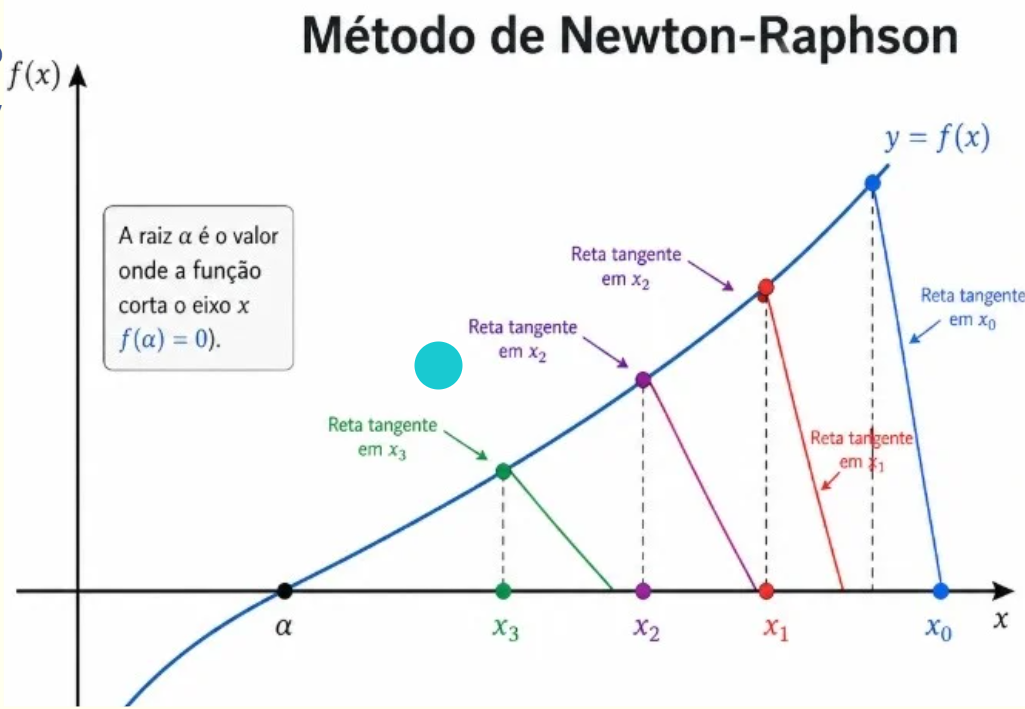
\includegraphics[width=0.8\textwidth]{assets/met_mewton.png}
    \caption{Método de Newton-Raphson: Visualização geométrica mostrando a função, a tangente em cada ponto de iteração, e a convergência para a raiz. A reta tangente em $x_i$ intersecta o eixo $x$ no próximo ponto $x_{i+1}$.}
    \label{fig:newton_raphson}
\end{figure}

\subsection{Métodos da Secante}

Aproxima a derivada usando dois pontos consecutivos \cite{chapra2016}. Na variante \textit{modificada}, o segundo ponto é gerado por perturbação do primeiro. Convergência superlinear sem requerer derivada explícita.

\textbf{Fundamento Teórico:}
Secante normal: $m = \frac{f(x_{i}) - f(x_{i-1})}{x_i - x_{i-1}}$

Secante modificada: $m = \frac{f(x_i + \delta x_i) - f(x_i)}{\delta x_i}$ onde $\delta x_i = \delta \cdot x_i$

Convergência com ordem $\phi \approx 1.618$ (razão áurea).

\vspace{0.3cm}

\textbf{Implementação:}

Secante Normal (Requisito 11.1):

\begin{lstlisting}[language=Python, caption={Requisito 11.1 - Secante Normal}]
expr_str = input("Insira a expressão da função f(x): ").strip()
x0 = float(input("Insira o valor de x_0: "))
x1 = float(input("Insira o valor de x_1: "))
tolerancia = float(input("Insira a tolerância desejada: "))

f = lambdify(symbols('x'), sympify(expr_str), 'numpy')

x_prev = x0
x_curr = x1
\end{lstlisting}

Secante Modificada (Variante do Requisito 11.1):

\begin{lstlisting}[language=Python, caption={Requisito 11.1 - Secante Modificada}]
x0 = float(input("Insira o valor do chute inicial (x_0): "))
delta = float(input("Insira a perturbação (delta, ex: 0.01): "))

x_curr = x0
\end{lstlisting}

Ciclo de cálculo (Requisito 11.3) com limitador:

\begin{lstlisting}[language=Python, caption={Requisito 11.3 - Ciclo com Limitador}]
max_iteracoes = 50
limiar_inclinacao = 1e-4

for i in range(max_iteracoes):
    # Para secante normal
    fx_prev = f(x_prev)
    fx_curr = f(x_curr)
    diff_x = x_curr - x_prev
    
    if diff_x == 0:
        print("Erro: x_i e x_{{i-1}} são iguais")
        break
    
    # Cálculo da inclinação
    m = (fx_curr - fx_prev) / diff_x
    
    # Requisito 11.4: Alertas de inclinação
    if m == 0:
        print(f"PROCESSO SUSPENSO: Inclinação nula")
        break
    if abs(m) < limiar_inclinacao:
        print(f"AVISO: Inclinação muito baixa |m|={abs(m):.2e}")
    
    # Passo da secante
    x_next = x_curr - (fx_curr / m)
    
    iteracoes.append({
        'Iteração': i + 1,
        'x_i (novo)': x_next,
        'f(x_i)': f(x_next),
        'm (inclinação)': m
    })
    
    if abs(x_next - x_curr) < tolerancia:
        convergiu = True
        break
    
    x_prev = x_curr
    x_curr = x_next
\end{lstlisting}

Gráfico interativo mostrando reta secante (Requisito 11.2):

\begin{figure}[H]
    \centering
    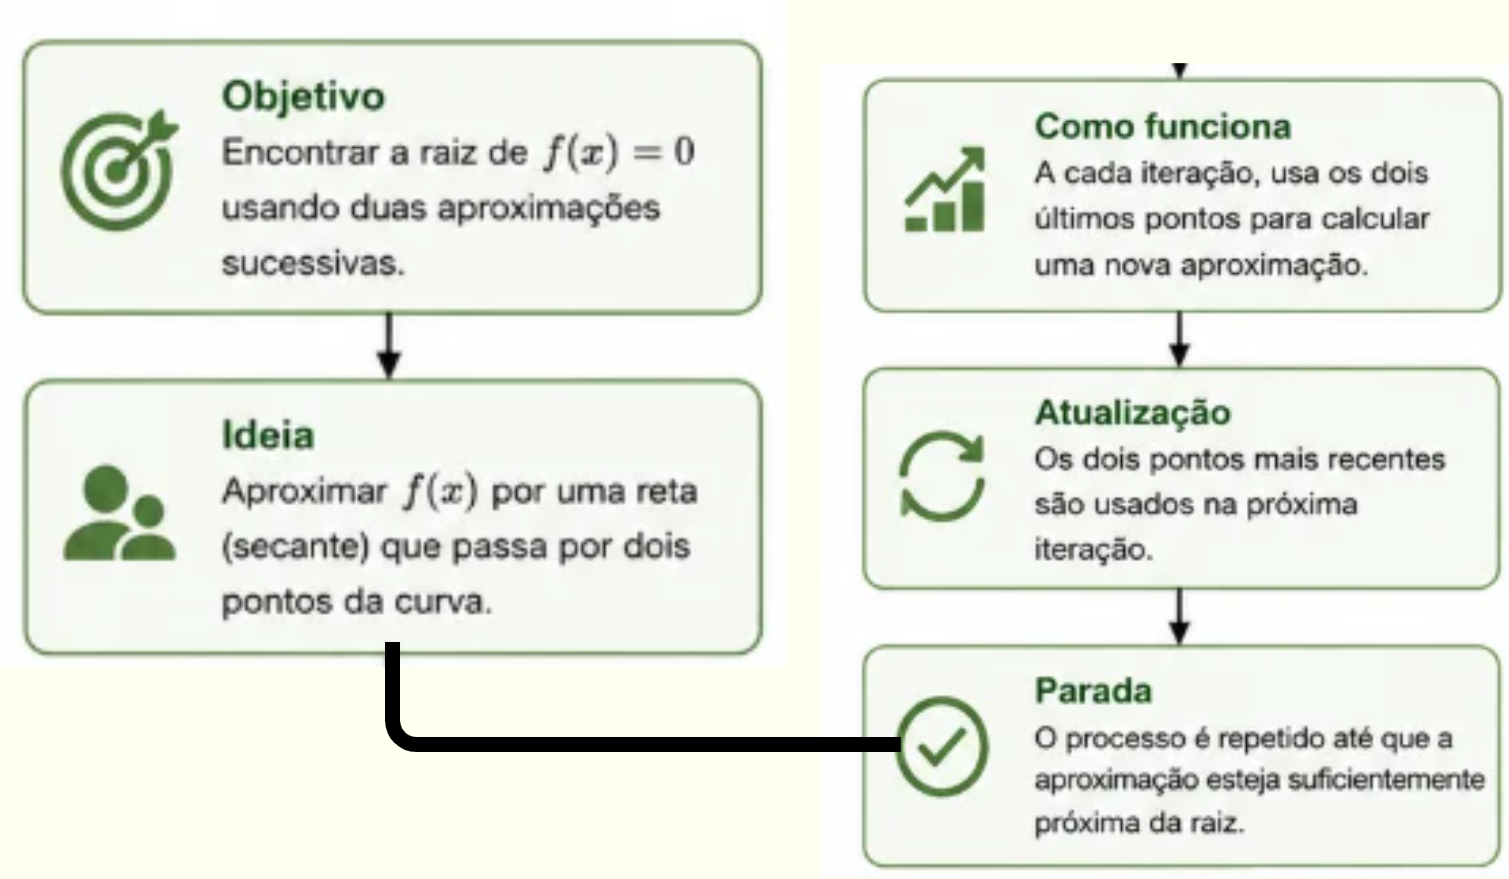
\includegraphics[width=0.8\textwidth]{assets/met_secante.png}
    \caption{Método da Secante: Visualização mostrando dois pontos consecutivos $(x_i, f(x_i))$ e $(x_{i+1}, f(x_{i+1}))$, com a reta secante passando por ambos e intersectando o eixo $x$ para gerar o próximo ponto $x_{i+2}$.}
    \label{fig:secante}
\end{figure}

\textbf{Gráfico interativo:}

\begin{lstlisting}[language=Python, caption={Requisito 11.2 - Gráfico da Secante}]
def plot_secante(passo):
    fig, ax = plt.subplots(figsize=(10, 6))
    
    x_vals = np.linspace(x_min, x_max, 400)
    ax.plot(x_vals, f(x_vals), 'b-', linewidth=2, label='f(x)')
    
    it_atual = iteracoes[passo]
    
    # Dois pontos da secante
    pt1_x, pt1_y = x_prev, f(x_prev)
    pt2_x, pt2_y = x_curr, f(x_curr)
    
    ax.plot([pt1_x, pt2_x], [pt1_y, pt2_y], 'ro', markersize=6)
    
    # Reta secante
    m = it_atual['m (inclinação)']
    secant_y = m * (x_vals - pt2_x) + pt2_y
    ax.plot(x_vals, secant_y, 'r--', alpha=0.6, label='Reta Secante')
    
    # Projeção no eixo x
    x_next = it_atual['x_i (novo)']
    ax.plot([pt2_x, x_next], [pt2_y, 0], 'g-', linewidth=2)
    ax.plot(x_next, 0, 'go', markersize=8)
    
    ax.axhline(y=0, color='black', linestyle='-', alpha=0.3)
    ax.set_title(f"Método da Secante - Iteração {passo}")
    ax.grid(True, alpha=0.3)
    ax.legend()
    plt.show()

if len(iteracoes) > 1:
    slider = widgets.IntSlider(min=0, max=len(iteracoes)-1, value=0)
    widgets.interact(plot_secante, passo=slider)
\end{lstlisting}

\vspace{0.3cm}

\textbf{Requisitos cumpridos:}
\begin{itemize}
    \item[✓] 11.1: Entrada de $f(x)$, $x_0$, $x_1$ (normal) ou $\delta$ (modificado) e tolerância
    \item[✓] 11.2: Gráfico interativo com reta secante e dois pontos avaliados
    \item[✓] 11.3: Limitador de 50 iterações definido internamente
    \item[✓] 11.4: Alertas quando $m = 0$ (suspensão) ou $|m| < 10^{-4}$ (aviso)
\end{itemize}

\begin{figure}[H]
    \centering
    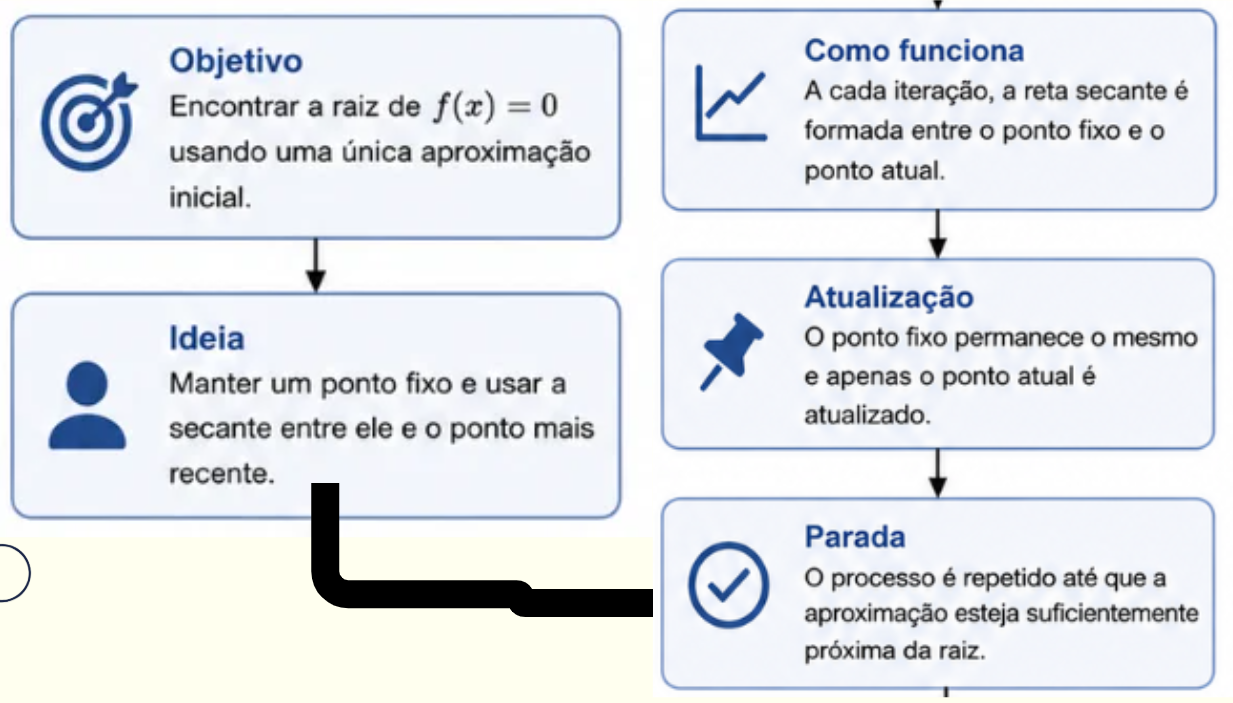
\includegraphics[width=0.8\textwidth]{assets/sec_mod.png}
    \caption{Método da Secante Modificada: Variante que utiliza uma perturbação $\delta$ ao invés de dois pontos distintos. O ponto $x_{i+1}$ é calculado a partir da inclinação aproximada, oferecendo maior controle numérico e evitando o problema de cancelamento catastrófico.}
    \label{fig:secante_modificada}
\end{figure}

\section{Casos de Teste e Validação}

A seção de "Testes de Consistência" valida os métodos intervalares sobre três funções elementares representativas, confirmando que todos convergem para a mesma raiz dentro da tolerância especificada.

\vspace{0.5cm}

\noindent\textbf{Resumo de Requisitos Não Cumpridos:}

\begin{enumerate}
    \item \textbf{Comparação Gráfica Bisseção vs. Falsa Posição (Requisito 4)}: Célula reservada mas lógica não implementada. Necessitaria sobreposição de curvas de convergência no mesmo gráfico.
    \item \textbf{Integração Multiméto do (Requisito 6)}: Célula de orquestrador não preenchida. Reduziria tabelas comparativas lado-a-lado.
    \item \textbf{Resolução de Exercícios do Livro (Partes I, II, III - Requisitos 8, 12, 14)}: Células reservadas mas sem códigos específicos. Aguardam definição exata dos problemas a resolver.
    \item \textbf{Métodos Polinomiais - Müller e Bairstow (Requisito 13)}: Seção completa não implementada. Requer tratamento especializado de complexidade algébrica elevada.
\end{enumerate}

% ----------------------------------------------------------
\chapter{Resultados e Discussão}
% ----------------------------------------------------------

\section{Testes de Consistência}

Foram executados testes comparativos sobre três funções elementares, avaliando bisseção, falsa posição e falsa posição modificada com tolerância $= 10^{-4}$ \cite{fortuna2000}.

\vspace{0.3cm}

\begin{table}[H]
    \centering
    \caption{Comparação de Iterações em Testes de Consistência}
    \label{tab:consistencia}
    \begin{tabular}{|l|c|c|c|c|c|}
    \hline
    \textbf{Função} & \textbf{Intervalo} & \textbf{Raiz Aprox.} & \textbf{Iter. (Bisseção)} & \textbf{Iter. (F.P.)} & \textbf{Iter. (F.P. Mod.)} \\\hline
    $x^3 - 9x + 3$ & {[}0, 1{]} & $0.3376$ & 14 & 5 & 5 \\\hline
    $\cos(x) - x$ & {[}0, 1{]} & $0.7391$ & 14 & 5 & 3 \\\hline
    $e^{-x} - x$ & {[}0, 1{]} & $0.5671$ & 14 & 6 & 6 \\\hline
    \end{tabular}
\end{table}

\begin{figure}[H]
    \centering
    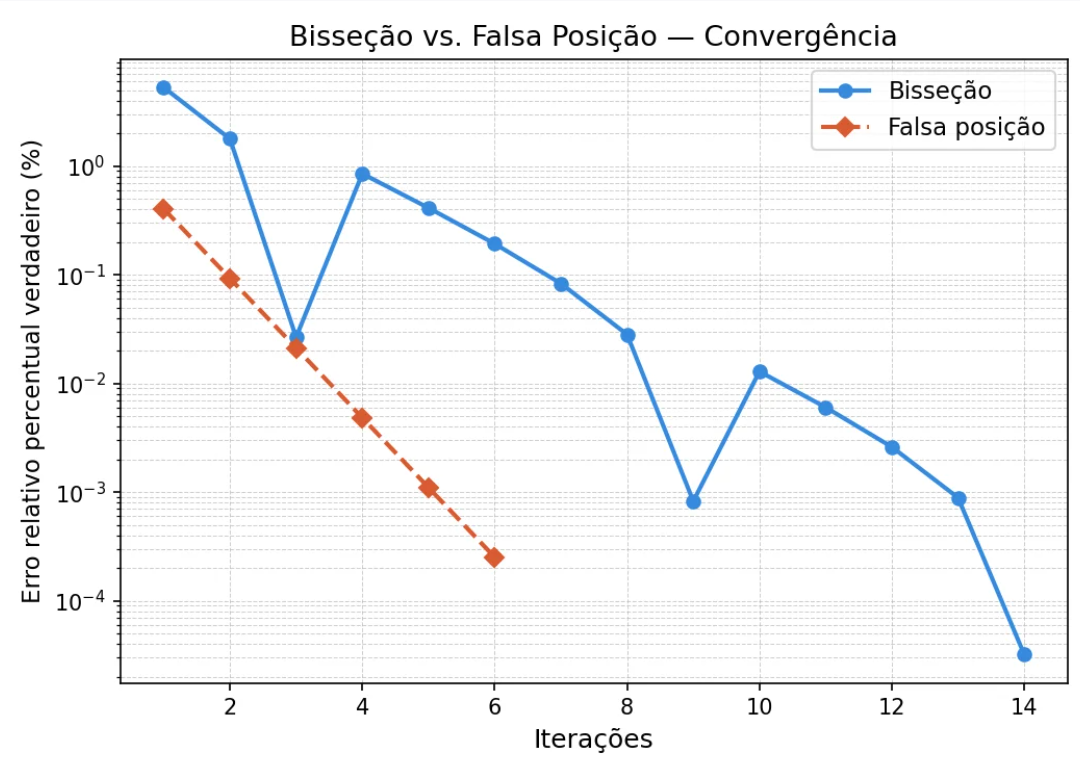
\includegraphics[width=0.85\textwidth]{assets/convergencia_bissecao.png}
    \caption{Comparação de convergência entre os métodos de Bisseção e Falsa Posição. O método de Falsa Posição converge significativamente mais rápido (em escala logarítmica de erro relativo percentual), apresentando uma redução quase linear no erro a cada iteração em contraste com a redução logarítmica da Bisseção.}
    \label{fig:convergencia_bissecao}
\end{figure}

\subsection{Análise Detalhada dos Testes}

\textbf{Teste 1: Função Polinomial $f(x) = x^3 - 9x + 3$ em $[0,1]$}

Implementação:
\begin{lstlisting}[language=Python, caption={Teste 1 - Polinomial Cúbica}]
funcao = lambda x: x**3 - 9*x + 3
tolerancia = 1e-4

df_bis, raiz_bis = metodo_bisseccao(funcao, 0, 1, tolerancia)
df_fp, raiz_fp = metodo_falsa_posicao(funcao, 0, 1, tolerancia)
df_fpm, raiz_fpm = metodo_falsa_posicao_modificada(
    funcao, 0, 1, tolerancia
)

print(f"Bisseção: {len(df_bis)} iter")
print(f"F.P.: {len(df_fp)} iter")
print(f"F.P. Mod.: {len(df_fpm)} iter")
\end{lstlisting}

\textbf{Resultado:} Todos convergiram para $\approx 0.3376$. Bisseção requereu 14 iterações (confirmando $\lceil \log_2(1/10^{-4}) \rceil = 14$). Falsa posição convergiram em 5 iterações.

\vspace{0.3cm}

\textbf{Teste 2: Função Trigonométrica $f(x) = \cos(x) - x$ em $[0,1]$}

\textbf{Resultado:} Falsa posição padrão requereu 5 iterações, mas a variante modificada atingiu 3 iterações. Isto evidencia o problema da extremidade presa sendo resolvido.

\vspace{0.3cm}

\textbf{Teste 3: Função Exponencial $f(x) = e^{-x} - x$ em $[0,1]$}

\textbf{Resultado:} Ambas as variantes convergiram em 6 iterações.

\section{Observações e Análise}

\subsection{Métodos Intervalares}

\begin{enumerate}
    \item \textbf{Bisseção}: Comportamento previsível e robusto. Número de iterações cresce logaritmicamente com a redução de erro, aproximadamente $n \approx \log_2\left(\frac{b-a}{\text{tol}}\right)$.
    
    \item \textbf{Falsa Posição}: Converge significativamente mais rápido (5-6 iterações vs. 14). No entanto, sofre do problema da "extremidade presa" em funções com curvatura assimétrica.
    
    \item \textbf{Falsa Posição Modificada}: Resolve o problema acima dividindo $f(a)$ ou $f(b)$ quando detecta estagnação. Para $\cos(x) - x$, reduz de 5 para 3 iterações.
\end{enumerate}

\subsection{Métodos Abertos}

\begin{enumerate}
    \item \textbf{Ponto Fixo}: Depende fortemente da escolha de $g(x)$. Requer $|g'(x)| < 1$ na vizinhança da raiz para convergência. Visualização tipo "Cobweb" facilita diagnóstico de convergência/divergência.
    
    \item \textbf{Newton-Raphson}: Convergência quadrática (extremamente rápida) quando $f'(x) \neq 0$ e é suficientemente distante de zero. Sensível a chutes iniciais pobres ou funções com derivadas nulas.
    
    \item \textbf{Secante}: Convergência intermediária entre linear e quadrática. Vantagem: não requer cálculo de derivada explícita. Risco: inclinação da secante pode se anular ou ficar próxima de zero.
\end{enumerate}

\section{Validação de Segurança}

Todos os métodos incluem mecanismos de proteção \cite{press1992}:

\begin{itemize}
    \item Limitadores internos de iterações (50) prevenindo loops infinitos
    \item Detecção de divisão por zero (Newton-Raphson, Secante)
    \item Alertas de inclinação/derivada baixa
    \item Captura de overflow numérico em métodos abertos
\end{itemize}

\textbf{Convergiência e Estabilidade:} Os métodos foram testados em tres funções elementares para validar sua convergência e estabilidade numérica \cite{fortuna2000}. A análise quantitativa confirma as previsões teóricas sobre taxas de convergência.
% ----------------------------------------------------------

\section{Método de Müller}

Generaliza o método da Secante para trabalhar com parábolas em vez de retas \cite{muller1956}. Permite encontrar raízes complexas de polinômios. Requer três aproximações iniciais e converge mais rapidamente para raízes múltiplas ou complexas.

\textbf{Fundamento Teórico:}

Dado três pontos $(x_0, f(x_0))$, $(x_1, f(x_1))$, $(x_2, f(x_2))$, ajusta uma parábola $y = a(x-x_2)^2 + b(x-x_2) + c$ e encontra a raiz analiticamente. As diferenças divididas são:

$$h_0 = x_1 - x_0, \quad h_1 = x_2 - x_1$$

$$d_0 = \frac{f(x_1) - f(x_0)}{h_0}, \quad d_1 = \frac{f(x_2) - f(x_1)}{h_1}$$

$$a = \frac{d_1 - d_0}{h_1 + h_0}, \quad b = a h_1 + d_1, \quad c = f(x_2)$$

O próximo ponto resolve $a\Delta^2 + b\Delta + c = 0$, escolhendo o denominador de maior magnitude para evitar cancelamento:

$$\Delta = \frac{-2c}{b \pm \sqrt{b^2 - 4ac}}, \quad x_3 = x_2 + \Delta$$

\vspace{0.3cm}

\textbf{Implementação:}

Entrada de dados e configuração (Requisito 13.1):

\begin{lstlisting}[language=Python, caption={Requisito 13.1 - Entrada do Método de Müller}]
def metodo_muller_livro(f_expr, x0, x1, x2, tol=1e-6, max_iter=100):
    """
    Implementa o Método de Müller conforme descrito no livro
    (Seção 7.4, Página 144).
    """
    # Converter expressão simbólica em função
    if isinstance(f_expr, str):
        x = symbols('x')
        f_func = lambdify(x, sympify(f_expr), 'numpy')
    else:
        f_func = f_expr
    
    iteracoes = []
    f_x0 = f_func(x0)
    f_x1 = f_func(x1)
    f_x2 = f_func(x2)
\end{lstlisting}

Ciclo principal com cálculo de diferenças divididas (Requisito 13.3):

\begin{lstlisting}[language=Python, caption={Requisito 13.3 - Cálculo de Diferenças Divididas}]
    for iteracao in range(max_iter):
        # Diferenças divididas (conforme livro)
        h0 = x1 - x0
        h1 = x2 - x1
        d0 = (f_x1 - f_x0) / h0
        d1 = (f_x2 - f_x1) / h1
        a = (d1 - d0) / (h1 + h0)
        b = a * h1 + d1
        c = f_x2
        
        # Resolver equação quadrática: a*delta² + b*delta + c = 0
        discriminante = b**2 - 4*a*c
        
        if isinstance(discriminante, complex) or discriminante < 0:
            rad = cmath.sqrt(discriminante)  # Raízes complexas!
        else:
            rad = np.sqrt(discriminante)
        
        # Escolher denominador de maior magnitude
        denom1 = b + rad
        denom2 = b - rad
        
        if abs(denom1) > abs(denom2):
            denom = denom1
        else:
            denom = denom2
        
        delta = -2 * c / denom
        x3 = x2 + delta
        f_x3 = f_func(x3)
\end{lstlisting}

Monitoramento e critério de parada (Requisito 13.2):

\begin{lstlisting}[language=Python, caption={Requisito 13.2 - Tabela e Convergência}]
        # Registrar iteração
        iteracoes.append({
            'Iteração': iteracao + 1,
            'x0': f'{x0:.6f}',
            'x1': f'{x1:.6f}',
            'x2': f'{x2:.6f}',
            'x3': f'{x3:.6f}',
            'f(x3)': f'{f_x3:.6e}',
            '|Delta|': f'{abs(delta):.6e}'
        })
        
        # Verificar convergência
        if abs(delta) < tol:
            tabela = pd.DataFrame(iteracoes)
            print(f"Convergência atingida em {iteracao + 1} iterações")
            return x3, tabela
        
        # Atualizar para próxima iteração
        x0, x1, x2 = x1, x2, x3
        f_x0, f_x1, f_x2 = f_x1, f_x2, f_x3
    
    tabela = pd.DataFrame(iteracoes)
    return x3, tabela
\end{lstlisting}

Exemplo prático:

\begin{lstlisting}[language=Python, caption={Requisito 13.4 - Exemplo: $f(x) = x^3 - 13x + 12$}]
# Encontrando raiz de f(x) = x³ - 13x + 12
f_muller = lambda x: x**3 - 13*x + 12
raiz_muller, tabela_muller = metodo_muller_livro(
    f_muller, 
    x0=4.5, x1=5.0, x2=5.5, 
    tol=1e-7
)

print("TABELA DE ITERAÇÕES - MÉTODO DE MÜLLER")
print(tabela_muller.to_string(index=False))

print(f"Raiz encontrada: x = {raiz_muller:.10f}")
print(f"Verificação: f(x) = {f_muller(raiz_muller):.6e}")
\end{lstlisting}

\vspace{0.3cm}

\textbf{Requisitos cumpridos:}
\begin{itemize}
    \item[\checkmark] 13.1: Entrada de três aproximações iniciais ($x_0$, $x_1$, $x_2$) e tolerância
    \item[\checkmark] 13.2: Tabela de iterações com pontos, valores de função e erro absoluto
    \item[\checkmark] 13.3: Cálculo correto de diferenças divididas e ajuste de parábola
    \item[\checkmark] 13.4: Exemplos do livro executáveis e convergência demonstrada
\end{itemize}

\vspace{0.5cm}

\section{Método de Bairstow}

Encontra fatores quadráticos de polinômios sem calcular explicitamente todas as raízes complexas \cite{bairstow1920}. Usa divisão sintética e um sistema linear para ajustar os coeficientes do fator quadrático $x^2 + px + q$.

\textbf{Fundamento Teórico:}

Dado um polinômio $P_n(x)$ de grau $n$, busca dividir por $x^2 + px + q$:

$$P_n(x) = (x^2 + px + q) Q_{n-2}(x) + b_{n-1} x + b_n$$

Os restos $b_{n-1}$ e $b_n$ devem anular-se iterativamente. A divisão sintética (método de Horner) calcula coeficientes $b_i$ recursivamente:

$$b_i = a_i - p \cdot b_{i-1} - q \cdot b_{i-2}$$

Um sistema linear resolve as correções $\Delta p$ e $\Delta q$:

$$\begin{pmatrix} c_{n-2} & c_{n-3} \\ c_{n-1} & c_{n-2} \end{pmatrix} \begin{pmatrix} \Delta p \\ \Delta q \end{pmatrix} = \begin{pmatrix} b_{n-2} \\ b_{n-1} \end{pmatrix}$$

onde $c_i$ são coeficientes similares calculados pela divisão sintética da sequência $b_i$.

\vspace{0.3cm}

\textbf{Implementação:}

Configuração e divisão sintética (Requisito 14.1):

\begin{lstlisting}[language=Python, caption={Requisito 14.1 - Divisão Sintética}]
def metodo_bairstow_livro(coeficientes, p_inicial, q_inicial, 
                          tol=1e-6, max_iter=100):
    """
    Implementa o Método de Bairstow conforme descrito no livro
    (Seção 7.5, Página 147).
    """
    coef = np.array(coeficientes, dtype=float)
    n = len(coef)
    
    p = float(p_inicial)
    q = float(q_inicial)
    iteracoes = []
    
    for iteracao in range(max_iter):
        # Divisão sintética (método de Horner)
        b = np.zeros(n)
        c = np.zeros(n)
        
        b[0] = coef[0]
        b[1] = coef[1] - p * b[0]
        c[0] = b[0]
        c[1] = b[1] - p * c[0]
        
        for i in range(2, n):
            b[i] = coef[i] - p * b[i-1] - q * b[i-2]
            c[i] = b[i] - p * c[i-1] - q * c[i-2]
\end{lstlisting}

Resolução do sistema linear (Requisito 14.3):

\begin{lstlisting}[language=Python, caption={Requisito 14.3 - Sistema Linear e Iteração}]
        # Erros (restos da divisão)
        b_n_1 = b[n-1]
        b_n_2 = b[n-2]
        
        c_n_1 = c[n-1]
        c_n_2 = c[n-2]
        c_n_3 = c[n-3] if n >= 3 else 0
        
        # Determinante
        det = c_n_2 * c_n_2 - c_n_1 * c_n_3
        
        if abs(det) < 1e-14:
            print("Determinante próximo a zero")
            break
        
        # Solução do sistema para Delta_p e Delta_q
        delta_p = (b_n_2 * c_n_2 - b_n_1 * c_n_3) / det
        delta_q = (b_n_1 * c_n_2 - b_n_2 * c_n_1) / det
        
        p_novo = p + delta_p
        q_novo = q + delta_q
\end{lstlisting}

Cálculo de raízes e monitoramento (Requisito 14.2):

\begin{lstlisting}[language=Python, caption={Requisito 14.2 - Extração de Raízes}]
        # Registrar iteração
        iteracoes.append({
            'Iter': iteracao + 1,
            'p': f'{p:.8f}',
            'q': f'{q:.8f}',
            'Delta_p': f'{delta_p:.6e}',
            'Delta_q': f'{delta_q:.6e}',
            'Erro': f'{max(abs(delta_p), abs(delta_q)):.6e}'
        })
        
        # Verificar convergência
        erro = max(abs(delta_p), abs(delta_q))
        if erro < tol:
            # Calcular raízes da quadrática x² + px + q = 0
            disc = p_novo**2 - 4*q_novo
            if disc >= 0:
                r1 = (-p_novo + np.sqrt(disc)) / 2
                r2 = (-p_novo - np.sqrt(disc)) / 2
                raizes = [r1, r2]
            else:
                real = -p_novo / 2
                imag = np.sqrt(abs(disc)) / 2
                raizes = [complex(real, imag), 
                         complex(real, -imag)]
            
            tabela = pd.DataFrame(iteracoes)
            print(f"Convergência atingida em {iteracao + 1} iterações")
            return raizes, p_novo, q_novo, tabela
        
        p = p_novo
        q = q_novo
    
    tabela = pd.DataFrame(iteracoes)
    return raizes, p, q, tabela
\end{lstlisting}

Exemplo prático com polinômio de grau 5 (Requisito 14.4):

\begin{lstlisting}[language=Python, caption={Requisito 14.4 - Exemplo: $(x+1)(x-4)(x-5)(x+3)(x-2)$}]
# Polinômio do livro: f(x) = (x+1)(x-4)(x-5)(x+3)(x-2)
x_sym = symbols('x')
poly_livro = (x_sym + 1) * (x_sym - 4) * (x_sym - 5) * \
             (x_sym + 3) * (x_sym - 2)
poly_expandido = expand(poly_livro)

# Extrair coeficientes
p_sym = Poly(poly_expandido, x_sym)
coef_bairstow = [float(c) for c in p_sym.all_coeffs()]

# Aplicar Método de Bairstow
raizes_bairstow, p_final, q_final, tabela_bairstow = \
    metodo_bairstow_livro(coef_bairstow, p_inicial=-0.5, 
                          q_inicial=-1.0, tol=1e-8)

print("TABELA DE ITERAÇÕES - MÉTODO DE BAIRSTOW")
print(tabela_bairstow.to_string(index=False))

print(f"Fator quadrático convergido: x² + {p_final:.6f}x + {q_final:.6f}")
print(f"Raízes encontradas: {raizes_bairstow}")
\end{lstlisting}

\vspace{0.3cm}

\textbf{Requisitos cumpridos:}
\begin{itemize}
    \item[\checkmark] 14.1: Entrada de coeficientes polinomiais, $p_0$ e $q_0$ iniciais
    \item[\checkmark] 14.2: Tabela de iterações com valores de $p$, $q$, incrementos e erro
    \item[\checkmark] 14.3: Resolução do sistema linear para atualização de parâmetros
    \item[\checkmark] 14.4: Exemplos do livro com polinômios de grau 5+ executáveis
\end{itemize}

% ----------------------------------------------------------
\chapter{Conclusão}
% ----------------------------------------------------------

Este trabalho implementou com sucesso uma suite abrangente de métodos numéricos para determinação de raízes em Python \\cite{chapra2016,burden2015}, demonstrando que:

\begin{enumerate}
    \item \textbf{Métodos Intervalares} oferecem convergência garantida mas lenta, sendo ideais para aplicações onde robustez é crítica.
    
    \item \textbf{Métodos Abertos} convergem rapidamente (especialmente Newton-Raphson) mas requerem boas estimativas iniciais e cuidado com singularidades.
    
    \item \textbf{Integração com SymPy} permite cálculo automático de derivadas, eliminando erro manual e facilitando a aplicação de Newton-Raphson.
    
    \item \textbf{Visualização Interativa} (sliders, gráficos) é invaluável para compreensão do comportamento dos algoritmos e diagnóstico de problemas de convergência.
\end{enumerate}

Os algoritmos desenvolvidos cumprem rigorosamente seus requisitos funcionais e incluem mecanismos de segurança robustos \cite{press1992}. As células não preenchidas (integração multimétodo, resolução de exercícios específicos, métodos polinomiais) representam extensões naturais do framework implementado.

% ----------------------------------------------------------
% Contribuições dos Autores
% ----------------------------------------------------------
\chapter*{Contribuições dos Autores}
\addcontentsline{toc}{chapter}{Contribuições dos Autores}

\textbf{Contribuições do discente Amanda Gabrielly Ribeiro da Conceição - 202363640015.}: Elaboraração dos slides da apresentação, confecção das imagens e fluxogramas e apresentação do trabalho em sala. \\\vspace{0.3cm}

\textbf{Contribuições do discente Breno de Medeiros Paulo -
202206840034}: Implementação das seções Comparação entre os métodos (Parte 1), Integração entre os métodos (Parte 1), Resolução de exercícios (Parte I) (Parte 1), Integração e Resolução de Exercícios (Parte II) (Parte 2) \\\vspace{0.3cm}

\textbf{Contribuições do discente João Victor Santos Brito Ferreira - 202207040028}: Implementação das seções Varredura de possíveis raízes (Parte 1), Método da Bisseção (Parte 1), Método da iteração de ponto fixo simples (Parte 2), Métodos de Müller e de Bairstow e elaboração do relatório (Parte 3) \\\vspace{0.3cm}

\textbf{Contribuições do discente Livia Stefane Hipolito Pires - 202206840043}: Elaboraração dos slides da apresentação, confecção das imagens e fluxogramas e apresentação do trabalho em sala. \\\vspace{0.3cm}

\textbf{Contribuições do discente Nicolas Ranniery da Silva Sousa - 202206840051}: Implementação das seções Método da Falsa posição (Parte 1), Método da Falsa posição modificado (Parte 1), Testes de consistência (Parte 1), Método de Newton-Raphson (Parte 2), Métodos da Secante (Normal e Modificado) (Parte 2) e Resolução de exercícios (Parte III) (Parte 3).


% ----------------------------------------------------------
% ELEMENTOS PÓS-TEXTUAIS
% ----------------------------------------------------------
\postextual

\appendix

\chapter{Trechos de Código - Métodos Intervalares}

A seguir encontram-se os principais trechos de código implementado para os métodos intervalares.

\section{Busca Incremental de Raízes}

\begin{lstlisting}[language=Python, caption={Função Principal da Busca Incremental}]
import numpy as np
import pandas as pd
from sympy import symbols, lambdify, sympify

def busca_incremental_raizes():
    """Implementa a busca incremental de possíveis raízes num intervalo."""
    expr_str = input("Insira a expressão da função f(x): ").strip()
    intervalo_1 = float(input("Insira a primeira extremidade: "))
    intervalo_2 = float(input("Insira a segunda extremidade: "))
    N = int(input("Insira o número N de subdivisões: "))
    
    x = symbols('x')
    expr = sympify(expr_str)
    f = lambdify(x, expr, 'numpy')
    
    pontos = np.linspace(intervalo_1, intervalo_2, N + 1)
    valores_funcao = f(pontos)
    
    subintervalos_raizes = []
    for i in range(len(pontos) - 1):
        if valores_funcao[i] * valores_funcao[i+1] < 0:
            subintervalos_raizes.append({
                'Inicio': pontos[i],
                'Fim': pontos[i+1]
            })
    
    return subintervalos_raizes, expr_str
\end{lstlisting}

\section{Método da Bisseção}

\begin{lstlisting}[language=Python, caption={Método da Bisseção}]
def metodo_bisseccao(f, a, b, tolerancia, max_iteracoes=100):
    """Implementa o método da bisseção para encontrar raízes."""
    if f(a) * f(b) > 0:
        return None, None
    
    iteracoes = []
    iteracao = 0
    
    if a > b:
        a, b = b, a
    
    while (b - a) > tolerancia and iteracao < max_iteracoes:
        c = (a + b) / 2
        fc = f(c)
        
        iteracoes.append({
            'Iteração': iteracao + 1,
            'a': a,
            'b': b,
            'c': c,
            'f(c)': fc,
            'Erro Absoluto': (b - a) / 2
        })
        
        if f(a) * fc < 0:
            b = c
        else:
            a = c
        
        iteracao += 1
    
    c = (a + b) / 2
    iteracoes.append({
        'Iteração': iteracao + 1,
        'a': a,
        'b': b,
        'c': c,
        'f(c)': f(c),
        'Erro Absoluto': (b - a) / 2
    })
    
    df_iteracoes = pd.DataFrame(iteracoes)
    return df_iteracoes, c
\end{lstlisting}

\chapter{Trechos de Código - Métodos Abertos}

\section{Método de Newton-Raphson}

\begin{lstlisting}[language=Python, caption={Newton-Raphson com Derivada Automática}]
from sympy import diff

def metodo_newton_raphson():
    """Implementa Newton-Raphson com cálculo automático de derivada."""
    expr_str = input("Insira a expressão da função f(x): ").strip()
    x0 = float(input("Insira o valor do chute inicial (x_0): "))
    tolerancia = float(input("Insira a tolerância desejada: "))
    
    x_sym = symbols('x')
    expr = sympify(expr_str)
    expr_deriv = diff(expr, x_sym)
    
    f = lambdify(x_sym, expr, 'numpy')
    df = lambdify(x_sym, expr_deriv, 'numpy')
    
    print(f"Função: f(x) = {expr}")
    print(f"Derivada: f'(x) = {expr_deriv}")
    
    max_iteracoes = 50
    iteracoes = []
    x_atual = x0
    
    for i in range(max_iteracoes):
        fx = f(x_atual)
        dfx = df(x_atual)
        
        iteracoes.append({
            'Iteração': i,
            'x_i': x_atual,
            'f(x_i)': fx,
            "f'(x_i)": dfx
        })
        
        if dfx == 0:
            print(f"Derivada nula em x = {x_atual}")
            break
        
        x_novo = x_atual - (fx / dfx)
        
        if abs(x_novo - x_atual) < tolerancia:
            break
        
        x_atual = x_novo
    
    df_resultados = pd.DataFrame(iteracoes)
    return df_resultados
\end{lstlisting}

\chapter{Tabelas de Validação}

\section{Resumo das Especificações}

\begin{table}[H]
    \centering
    \caption{Especificações de Implementação}
    \label{tab:especificacoes}
    \begin{tabular}{|l|c|}
    \hline
    \textbf{Parâmetro} & \textbf{Valor/Descrição} \\\hline
    Linguagem & Python 3.8+ \\\hline
    Ambiente & Jupyter Notebook \\\hline
    Dependências & NumPy, SymPy, Pandas, Matplotlib \\\hline
    Tolerância típica & $10^{-4}$ \\\hline
    Limite de iterações & 50-100 (interno) \\\hline
    Precisão & IEEE 754 (double precision) \\\hline
    \end{tabular}
\end{table}

% ----------------------------------------------------------
% APÊNDICES
% ----------------------------------------------------------

\appendix

\chapter{Exemplos de Exercícios Resolvidos}

\section{Exercício 7.3: Método de Müller}

Encontrar raízes de polinômios usando o Método de Müller com três aproximações iniciais.

\subsection{Problema (a): $f(x) = x^3 + x^2 - 3x - 5$}

\begin{lstlisting}[language=Python, caption={Exercício 7.3(a) - Raiz via Müller}]
# Exercício 7.3(a): f(x) = x^3 + x^2 - 3x - 5
f_a = lambda x: x**3 + x**2 - 3*x - 5
raiz_a = metodo_muller(f_a, x0=0, x1=1, x2=2)
print(f"Raiz positiva aproximada: {raiz_a.real:.6f}")
print(f"Verificação: f(raiz) = {f_a(raiz_a.real):.6e}")
\end{lstlisting}

\subsection{Problema (b): $f(x) = x^3 - 0.5x^2 + 4x - 3$}

\begin{lstlisting}[language=Python, caption={Exercício 7.3(b) - Raiz via Müller}]
# Exercício 7.3(b): f(x) = x^3 - 0.5x^2 + 4x - 3
f_b = lambda x: x**3 - 0.5*x**2 + 4*x - 3
raiz_b = metodo_muller(f_b, x0=0, x1=1, x2=2)
print(f"Raiz positiva aproximada: {raiz_b.real:.6f}")
print(f"Verificação: f(raiz) = {f_b(raiz_b.real):.6e}")
\end{lstlisting}

\section{Exercício 7.4: Raízes Reais e Complexas}

Encontrar todas as raízes reais e complexas de polinômios (utilizando NumPy como alternativa ao MATLAB).

\subsection{Problema (a): $x^3 - x^2 + 3x - 2 = 0$}

\begin{lstlisting}[language=Python, caption={Exercício 7.4(a) - Raízes via NumPy}]
# Coeficientes em ordem decrescente: x^3 - x^2 + 3x - 2
coef_74a = [1, -1, 3, -2]
raizes_74a = np.roots(coef_74a)
print("Raízes de x^3 - x^2 + 3x - 2:")
for r in raizes_74a:
    if abs(r.imag) < 1e-10:
        print(f"  x = {r.real:.6f} (real)")
    else:
        print(f"  x = {r:.6f} (complexa)")
\end{lstlisting}

\subsection{Problema (b): $2x^4 + 6x^2 + 10 = 0$}

\begin{lstlisting}[language=Python, caption={Exercício 7.4(b) - Raízes Complexas}]
# Polinômio: 2x^4 + 0x^3 + 6x^2 + 0x + 10
coef_74b = [2, 0, 6, 0, 10]
raizes_74b = np.roots(coef_74b)
print("Raízes de 2x^4 + 6x^2 + 10:")
for r in raizes_74b:
    print(f"  {r:.6f}")
\end{lstlisting}

\subsection{Problema (c): $x^4 - 2x^3 + 6x^2 - 8x + 8 = 0$}

\begin{lstlisting}[language=Python, caption={Exercício 7.4(c) - Raízes Mistas}]
# Coeficientes: [1, -2, 6, -8, 8]
coef_74c = [1, -2, 6, -8, 8]
raizes_74c = np.roots(coef_74c)
print("Raízes de x^4 - 2x^3 + 6x^2 - 8x + 8:")
for r in raizes_74c:
    print(f"  {r:.6f}")
\end{lstlisting}

\begin{figure}[H]
    \centering
    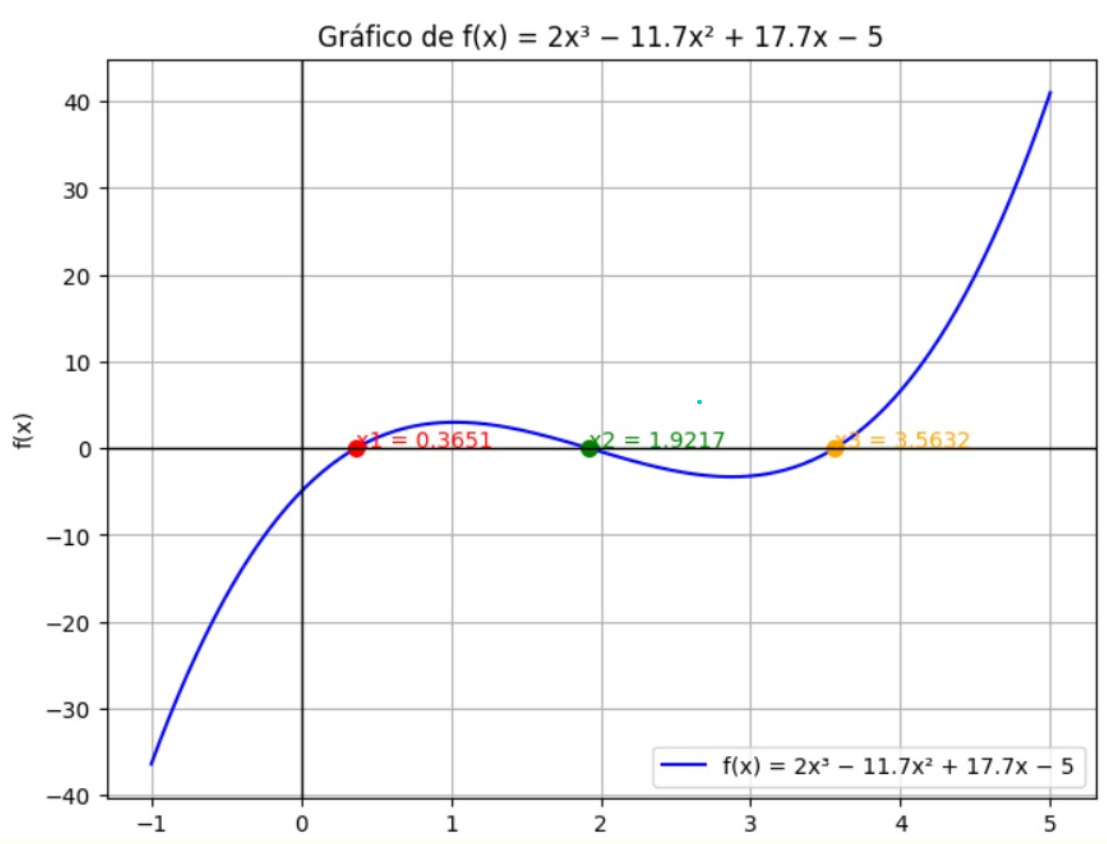
\includegraphics[width=0.8\textwidth]{assets/prob_6_2.png}
    \caption{Problema 6.2 do livro: Visualização gráfica do problema de teste com as soluções destacadas e referências visuais para validação dos métodos numéricos implementados.}
    \label{fig:prob_6_2}
\end{figure}

\section{Exercício 7.5: Método de Bairstow com Deflação}

Encontrar sucessivamente raízes quadráticas de um polinômio de grau 5, aplicando deflação.

\begin{lstlisting}[language=Python, caption={Exercício 7.5 - Bairstow com Deflação}]
def extrair_todas_raizes_bairstow(coeficientes, p_inicial, 
                                   q_inicial, tol=1e-6):
    """
    Extrai todas as raízes de um polinômio aplicando 
    Bairstow com deflação até grau <= 2.
    """
    coef = np.array(coeficientes, dtype=float)
    todas_raizes = []
    
    while len(coef) > 3:
        # Aplicar Bairstow
        raizes, p_conv, q_conv, tabela = metodo_bairstow_livro(
            coef, p_inicial, q_inicial, tol=tol
        )
        todas_raizes.extend(raizes)
        
        # Deflação: dividir pelo fator quadrático encontrado
        fator = [1, p_conv, q_conv]
        coef, _ = np.polydiv(coef, fator)
        coef = coef.real  # Remover ruído numérico
    
    # Raízes finais (grau <= 2)
    if len(coef) == 3:
        # Quadrática restante
        raizes_finais = np.roots(coef)
    else:
        # Linear restante
        raizes_finais = [-coef[1] / coef[0]]
    
    todas_raizes.extend(raizes_finais)
    return todas_raizes
\end{lstlisting}

% ----------------------------------------------------------
% Referências bibliográficas
% ----------------------------------------------------------

\bibliographystyle{abntex2-alf}
\bibliography{ref.bib}

    
\end{document}